\section{A \SU{2} model -- strongly interacting Grassmann numbers}\label{sec:0dSU2}
\begin{disclaimer}
	This section is based on the draft~\cite{Steil:partIV} and related ongoing work. So far the main contributions to this work have come from Adrian Koenigstein and Jens Braun. The complete set of flow equations for the field-dependent couplings is original to this thesis.
	
	The automated symbolic computations, full expressions, and the code for diagram generation and export are included in the digital auxiliary file~\cite{Steil:2023zeroDSU2} which relies heavily on 
	our \WAM{} code~\cite{Steil:2023PhDFlowEquationsNB} for flow equations. These symbolic computations, including the export of diagrams and \LaTeX{} expressions, take a few minutes on an \intel{} running multi-threaded on up to six cores.
\end{disclaimer}
\renewcommand{\FSk}{t}
So far in our studies of theories in zero dimensions we have only considered scalar degrees of freedom. 
Fermionic and Fermion-Boson models and theories, like the \qmm{} and \gnm{}, including \gmv{} fields are at the core of our research in \cref{chap:GN,chap:QMM}. 
This is why the wish to study fermions in zero dimensions, \ie{}, just Grassmann numbers, arose very early in our research project in zero dimensions.

Early on in our work on the manuscript for \ccite{zerod1}, we considered an extension of the $O(N=3)$ model by coupling it with four Grassmann numbers \dash{} an associated pair of Grassmann numbers with two flavors. 
The idea was to construct a simple $SU(2)$-symmetric model as a zero-dimensional analog to a Yukawa theory/\qm{}-like model.
We will present the construction of such a theory in \cref{subsec:0dSU2model}.
The corresponding \frg{} flow equations will be discussed in \cref{subsec:0dSU2flowEqs}.
The hope is, that such a more involved zero-dimensional theory would be suited to study more interesting symmetry breaking and restoration patterns than the one realized in the zero-dimensional $O(N)$ model.
In the zero-dimensional $O(N)$ model one can only study symmetry restoration by specifying an initial condition for the \frg{} flow which has a non-trivial minimum and study its evaporation during the \frg{} flow, see, \eg{}, \cref{subsec:0dONresults}.
The Grassmann-numbers of our $SU(2)$ model manifest as a source/sink-term in the flow equation for the \rgscaledependent{} potential, as we will demonstrate in \cref{paragraph:0dSU2flowU}.
This is a feature they share with fermionic contributions in higher dimensions, which also manifest as source/sink-like contributions in \lpa{} flow equations, \cf{} \cref{subsec:lpaDSeq}.
The hope is that such a source term would allow for a dynamically generated breaking of $SU(2)$ invariance in form of a precondensation effect, see also \cref{subsec:gnyFiniteNresults}.
While we still ultimately expect $SU(2)$ symmetry restoration in the \ir{} in zero-dimensions \dash{} due to the limiting case of the \cmwhTheoremWithRefs{}, \ie{}, basic symmetry-properties of the involved integrals \dash{} dynamic symmetry breaking and subsequent restoration during the \frg{} flow might be possible with a carefully constructed test cases.\bigskip

The work on this zero-dimensional $SU(2)$ model is still ongoing and we will only present some symbolic results, conceptual ideas and challenges in the following.
We have made only limited progress on this part of our research in zero dimensions from its conception in the early days of the manuscript for \ccite{zerod1} (in the fall of 2020) until now (fall of 2023) for various reasons:
\begin{itemize}
	\item We decided to work and publish our results for the $O(N)$ model as a ``first step''. 
	During our work on the $O(N)$ model in \dzero{} it turned out that this scalar theory alone is incredibly rich and the ``first step'' turned into a series of three publications~\cite{zerod1,zerod2,zerod3} covered in around 100 pages in this thesis, with still some open questions left.
	\item Applications of our results from this series~\cite{zerod1,zerod2,zerod3} to $d>0$, \cf{} \cref{chap:GN} and the corresponding preprint~\cite{Stoll:2021ori}, took precedence over further work in $d=0$.
	\item The constructed $SU(2)$ model in its non-bosonized, completely field-dependent form turned out to be diagrammatically rather complex.
	This complexity also manifests at the level of the flow equations, which presents an ambivalence.
	On the one hand, a conservative formulation (and related robust numerical implementation) of the involved flow equation has proven challenging and is still a work in progress.
	But on the other hand, this challenge in zero dimensions might be able to provide important insight into the conservative formulation of the \frg{} flow equation in general.
	The latter is very relevant for studies in higher dimensions, \eg{}, in with the \qmm{}, where a conservative formulation for the field-dependent Yukawa coupling is also still elusive~\cite{\consYRef}.	
\end{itemize}
We spent a lot of time developing code~\cite{Steil:2023PhDFlowEquationsNB,Steil:2023zeroDSU2} to derive, manipulate, and visualize diagrammatic flow equations.
We hope to use these tools in the future to gain further insight into the zero-dimensional $SU(2)$ model, or a simplified version of it.
We firmly believe that developing a better (or, in the best case, complete) understanding of zero-dimensional theories involving Grassmann numbers within the \frg{}-\cfd{} framework is a very promising research direction, with possibly significant implications beyond zero dimensions.
A part of the outlook~\ref{paragraph:0dconclusionFermions} for this chapter will be dedicated to discussing our plans and hopes for this research.

\subsection{Construction of the \SU{2} Grassmann-scalar theory}\label{subsec:0dSU2model}
\begin{disclaimer}
	This subsection is based on Sec.~II.A of the draft~\cite{Steil:partIV}.
	The main conceptual work in the explicit construction of the discussed model, based on symmetry considerations, has been done by Adrian Koenigstein.
\end{disclaimer}
\vspace{-.1em}
The aim of this subsection is to construct a preferably simple toy model for a consistent \qft{} in zero space-time dimensions, that contains bosonic and fermionic degrees of freedom, \ie{}, scalars and Grassmann-numbers.
We are interested in a theory, that has more than one scalar and more than one \gmv{} degree of freedom, to generate different types of contributions to the \frg{} flow equations.
We want a theory with convection-, diffusion-, and source/sink-like contributions in its \frg{} flow equations to mimic the situation found in the \lpa{}/\de{} of higher-dimensional theories, like the \gnm{} and \qmm{}, discussed in \cref{chap:GN,chap:QMM}.\clearpage

In addition, the model should allow for the possibility of the breakdown/restoration of a continuous symmetry and the formation of a condensate on the level of the \eaa{} $\FSeaa_t[\chi]$.
Such a dynamic symmetry breaking could be induced by attractive \gmv{} interactions during the \frg{} flow from $t = 0$ to $t \rightarrow \infty$.
The bosonic scalar degrees of freedom are however expected to restore the full symmetry and vaporize the condensate for the full quantum effective theory $\Gamma[\chi]$ in the deep infrared at $t \rightarrow \infty$, due to a limiting case of the \cmwhTheoremWithRefs{}, \cf{} \MWApp.
To allow for all these phenomena and to use them as testing tools, the action $S$ of the theory, to be constructed, has to be invariant under transformations of a continuous symmetry-group. 
To have a non-trivial \xcancel{field} theory, we include (self-)interaction terms in the action.
To enable interactions between scalar and \gmv{} degrees of freedom, we include a Yukawa-like coupling.
This inclusion also allows for the possibility of condensate formation and symmetry-breaking in $\FSeaa_t[\chi]$ during the \rg{}-flow.
All fermion self-interactions beyond a specific order must vanish due to the limited amount of distinct Grassmann numbers.

\paragraph{Grassmann numbers \dash{} the fermions in \texorpdfstring{\dzero{}}{d=0}}\phantomsection\label{paragraph:0dSU2modelFermions}\mbox{}\\%
We consider two anticommuting Grassmann numbers $\theta = (\theta^1 ,\, \theta^2 )$ and two associated anticommuting Grassmann numbers $\bar{\theta} = (\bar{\theta}_1 ,\, \bar{\theta}_2)$.
These tuples shall transform under the fundamental representation of a global $SU(N = 2)$ symmetry group,
		\begin{align}
			&	\theta \mapsto \theta^\prime = \suNU{}\, \theta \, ,	&&	\bar{\theta} \mapsto \bar{\theta}^\prime = \bar{\theta}\, \suNU{}^{ \dagger} \, ,	\label{eq:su2_fermion}
		\end{align}
	where
		\begin{align}
			&	\suNU{} = \eu^{+ \iu \vts{} \omega_a  \suIItup{a} } \, ,	&&	\suNU{}^{\dagger} = \eu^{-\iu\vts{} \omega_a  \suIItup{a} } \, ,	\label{eq:su_2_rotations}
		\end{align}
	with $a = 1,\,2,\,3$, the generators $\suIItup{a}$ of the group $SU(2)$ in fundamental representation forming the $\mathfrak{su}(2)$-algebra
		\begin{align}
			\big[ \suIIt{a} ,\, \suIIt{b} \big] =\, & \iu \, \lcs^{a b c}\suIIt{c}  \, ,	\label{eq:su2_lie_algebra}
		\end{align}
	\cf{} \cref{app:SU2} for further details and explicit expressions.
Using these Grassmann numbers, we can construct all contributions formed by $\Ftheta$ and $\Fthetab$ to the action $S$, which are invariant under $SU(2)$ symmetry.
From the transformation laws \eqref{eq:su2_fermion} we directly read off that there can not be any $SU(2)$-invariant terms involving only odd powers fermion flavors.
Furthermore, we find that there can only be a single term of fourth-order in fermion fields $\sim \bar{\theta}_1 \, \bar{\theta}_2 \, \theta^1 \, \theta^2$, because there are simply just four distinct Grassmann numbers available.
All higher-order terms vanish. 
Conventionally, we write the fourth-order term as
\begin{align}
	\frac{1}{2} \,g\, \big( \bar{\theta} \, \tfrac{1}{2} \, \Id_2 \, \theta \big)^2 = \frac{1}{8} \,g\, ( \bar{\theta} \, \theta )^2 = \frac{1}{4} \,g\, \bar{\theta}_1 \, \theta^1 \, \bar{\theta}_2 \, \theta^2 \, ,
\end{align}
with a four-Grassmann coupling constant $g$.

It remains to study the quadratic order terms: All possible terms are of the following form,
	\begin{align}
		\bar{\theta} \, M \, \theta \, ,	\label{eq:fermion_quadratic_interaction}
	\end{align}
where $M$ is a $2 \times 2$ complex matrix.
If this term is supposed to be invariant under the $SU(2)$ symmetry transformations \eqref{eq:su2_fermion}, assuming that $M$ does not transform itself under these symmetry transformations, then $M$ has to commutate with all fundamental generators \eqref{eq:SU2Tfundamental}. 
This implies that $M$ must be proportional to the only Casimir-operator of $SU(2)$, which is in turn proportional to the identity matrix:
\begin{align}
M =  \tfrac{1}{2}\, m \, \Id_2\,
\label{eq:0dSU2modelmDef}
\end{align}
with the coupling constant $m$, which we will typically refer to as ``mass function`` even though there is no notion of physical mass in \dzero{}.
Of course there is also the option that $M$ does not transform trivially under $SU(2)$, which we will discuss in the \customref{paragraph:0dSU2modelYukawa}{next-to-next paragraph} after discussing scalars first.

\paragraph{Scalars \dash{} the bosons in \texorpdfstring{\dzero{}}{d=0}}\phantomsection\label{paragraph:0dSU2modelBosons}\mbox{}\\%
We consider three scalars which are supposed to transform under the adjoint representation of $SU(2)$, thus forming a $SU(2)$-triplet.
We consider the components $(\phi_a) = (\phi_1 ,\, \phi_2 ,\, \phi_3)$ of a vector $\phi = \suIIta{a} \, \phi_a$, that transforms according to
	\begin{align}
		\phi_a \mapsto \phi^\prime_a = \suNU{}^{ab}\, \phi_b \, ,	\label{eq:adjoint_transformation}
	\end{align}
where
\begin{align}
	\suNU{}^{ab}\equiv (\exp(\iu \vts \omega_c\suIIta{c}))^{ab} \, ,	\label{eq:adjoint_group_elements}
\end{align}
with $a = 1,\, 2,\, 3$ and $\omega_a$ being the same group parameters as in \cref{eq:su_2_rotations}. 
The generators of $SU(2)$ in the adjoint representation $\suIIta{c}$, \cf{} \cref{eq:su2adjExp}, are given by the structure constant, $(\suIIta{a})^{b c}=-\iu \lcs^{a b c}$, which also form a basis of the Lie-algebra \eqref{eq:su2_lie_algebra}.
However, due to the double cover of $SU(2) \rightarrow SO(3)$, the adjoint representation maps elements of $SU(2)$ to the real vector representation of $SO(3)$.
Thus \cref{eq:adjoint_transformation} can also be written as the transformation of the components $\phi_a$ of an Euclidean vector $\phi$ under $SO(3)$-rotations
\begin{align}
	\phi_a \mapsto \phi^\prime_a = O_{a b} \, \phi_b \, ,
\end{align}
with
\begin{align}
	O = \eu^{ \iu \vts\omega_a L_a} \in SO(3) \, ,	\label{eq:so_3_rotation}
\end{align}
where $(L_b)_{ac} = -\iu\vts \varepsilon_{a b c}$ are the generators of three-dimensional rotations that coincide with $\suIIta{c}$.
	
From this, we can start to construct all scalar contributions to the action $S$, which are invariant under $SU(2)$ transformations, or the corresponding $SO(3)$ rotations respectively.
Naturally, all terms that are functions of the $SO(3)$ invariant
\begin{align}
	\rho \equiv \tfrac{1}{2} \, \phi_a \phi^a \label{eq:definition_so_3_invariantSU2}
\end{align}
must be included in the action of the theory.
This implies that for the purely scalar part of the action $S$, the only term that contributes and can be included in $S$, is the effective self-interaction potential $U(\rho)$, which we are familiar with from \cref{sec:0dON}.

It remains to study all $SU(2)$-invariant mixed interaction terms.
	
\paragraph{Grassmann-scalar interaction \dash{} the Yukawa coupling in \texorpdfstring{\dzero{}}{d=0}}\phantomsection\label{paragraph:0dSU2modelYukawa}\mbox{}\\%
To construct all possible $SU(2)$-invariant Grassmann-scalar interaction terms, we come back to the crucial observation, that all terms that are functions of $\rho$ are invariant under the $SO(3)$ symmetry transformations of the model. 
This implies that the first step is, to promote the two couplings $m$ and $g$ to field-dependent couplings $m(\rho)$ and $g(\rho)$, which maximally generalizes both terms, while keeping their symmetry untouched.
	
In the last step, it is sufficient to go back to the quadratic fermion interaction \eqref{eq:fermion_quadratic_interaction}.
This time, however, we allow for a non-trivial transformation behavior of $M$ under $SU(2)$,
\begin{align}
	\bar{\theta} \, M \, \theta \mapsto \bar{\theta}^\prime \, M^\prime \, \theta^\prime = \bar{\theta} \, \suNU{}^{\dagger} \, M^\prime \, \suNU{} \, \theta \,.
\end{align}
If we demand that the whole term should be invariant under $SU(2)$ transformations it follows that $M$ has to transform as ,
\begin{align}
	M \mapsto M^\prime = \suNU{} \, M \, \suNU{}^{\dagger} \,.	\label{eq:transformation_m}
\end{align}
This can of course be fulfilled trivially by a field-dependent mass-term $M \sim m(\rho) \, \bar{\theta} \, \tfrac{1}{2} \, \Id_2 \, \theta$, which we already included in the action ${S}$.
Additionally, \cref{eq:transformation_m} is exactly the transformation law that defines the adjoint representation.
We can therefore include another $SU(2)$-invariant term in the action $S$ that is quadratic in the fermion flavors,
\begin{align}
	\iu\vts h(\rho) \, \bar{\theta} \, T^{(\mathrm{f})}_a \, \phi_a \, \theta \, ,
\end{align}
where $h(\rho)$ is a field-dependent Yukawa-coupling.
The complex factor $\mathrm{i}$ is introduced for later convenience.\bigskip

In total, the most general action of the zero-dimensional $SU(2)$ model reads
	\begin{align}
		{S}[\vec{\phi},\theta,\bar{\theta}] = \, & U(\rho) + \bar{\theta} \, \big( \tfrac{m(\rho)}{2} \, \Id_2 + \mathrm{i}\, h(\rho) \, \suIIt{a}\, \phi_a \big) \, \theta + \tfrac{g(\rho)}{2} \, \big( \bar{\theta} \, \tfrac{1}{2} \, \Id_2 \, \theta \big)^2 \,.\label{eq:full_su2_action}
	\end{align}
	At this point, we remark, that in addition to the $SU(2)$ symmetry, the model exhibits a completely independent $U(1)$ symmetry, which manifests itself as pure phase-transformations of the fermion-fields, while the bosonic degrees of freedom stay unchanged,
		\begin{align}
			\bar{\theta} \mapsto \bar{\theta}^\prime = \bar{\theta} \, \eu^{ + \iu\vts \omega} \,,	\qquad	\theta \mapsto \theta^\prime = \eu^{ - \iu\vts \omega } \, \theta \,, \qquad	\phi_a \mapsto \phi^\prime_a = \phi_a \,.	\label{eq:global_u_1}
		\end{align}
	This is the zero-dimensional analog to the conservation of baryon number, \cf{} \cref{paragraph:qcdChiral}.
	
	Regarding the action \eqref{eq:global_u_1} two issues remain to be discussed: Firstly, we have to discuss the symmetry breaking/restoration pattern, which can emerge dynamically during the \frg{} flow in $\bar{\Gamma}_t[\chi]$. Secondly, we have to discuss the restrictions on the functions $m(\rho)$, $h(\rho)$, $g(\rho)$, and $U(\rho)$ and if they have to be chosen real or complex valued. 
	The action $S$ of our model should be real-valued, to allow for an interpretation as a probability distribution.

\paragraph{Symmetry breaking/restoration pattern}\phantomsection\label{paragraph:0dSU2modelSym}\mbox{}\\%
The possible symmetry breaking/restoration pattern at finite \rgtime{} $t$ comprises:
The $SU(2)$ symmetry can only break down to one of its $U(1)$subgroups, if we want to end up in a continuous subgroup with ``Goldstone-modes'', \cf{} \cref{subsec:symmetry_restoration}, because there are no other continuous subgroups of $SU(2)$.
In the bosonic sector, this $SU(2)$ symmetry breaking corresponds to a symmetry breaking of $SO(3)$ to one of its continuous $SO(2)$ subgroups, thus it total, the breaking pattern is given by
\begin{align}
	U(1) \otimes SU(2) \rightarrow \, & U(1) \otimes U(1) \, ,\\[0.1em]
	SO(3) \rightarrow \, & SO(2) \, .
\end{align}
On the level of the \eaa{} $\FSeaa_t[\chi]$ this is realized as follows: During the dynamical symmetry breaking, a condensate $\sigma$ and two ``Goldstone-modes'' $\pi_1$ and $\pi_2$ are formed. The number of ``Goldstone-modes'' is given by the number of broken generators of the symmetry group $SO(3)$, which is two, if we end up with a $SO(2)$ symmetry, that has only one remaining generator. 
Because there is no external parameter that distinguishes a single field space direction in $\phi$ from the other directions (because we do not consider explicit symmetry breaking), we can choose any of the field directions as the direction of the condensate $\sigma$.
Without loss of generality, we choose $\phi_3$ as the direction of condensation and $\phi_1$ and $\phi_2$ as the pion directions $\pi_1$ and $\pi_2$.
This implies that the remainder $SO(2)$ symmetry corresponds to rotations in the $\phi_1$-$\phi_2$-plane in field space, which leaves the condensate $\phi_3 = \sigma$ invariant.
This is obtained by setting $\omega_{1} =\omega_{2}= 0$ in \cref{eq:so_3_rotation},
\begin{align}
	&	\phi_a \mapsto \phi^\prime_a = O_{a b} \, \phi_b \,,	&&	O = \eu^{ \iu{}\vts{} \omega_3 L_3} \,,	\label{eq:o_2_rotation}
\end{align}
and explicitly reads
\begin{align*}
	\begin{pmatrix}
		\phi_1	\\
		\phi_2	\\
		\phi_3
	\end{pmatrix} \mapsto
	\begin{pmatrix}
		\phi^\prime_1	\\
		\phi^\prime_2	\\
		\phi^\prime_3
	\end{pmatrix}
	=
	\begin{pmatrix}
		\cos(\omega_3)	&	\sin(\omega_3)	&	0	\\
		-\sin(\omega_3)	&	\cos(\omega_3)		&	0	\\
		0				&	0					&	1
	\end{pmatrix}
	\begin{pmatrix}
		\phi_1	\\
		\phi_2	\\
		\phi_3
	\end{pmatrix} \,.
\end{align*}
Thus, we find that the $SO(3) \rightarrow SO(2)$ symmetry breaking is realized as a non-vanishing condensate $\sigma$ in one of the field space directions, which corresponds to a non-trivial minimum $\rho=\underline{\rho}=\tfrac{1}{2}\sigma^2>0$ in at least one of the field-dependent couplings $m(\rho)$, $g(\rho)$, $h(\rho)$ or the effective potential $U(\rho)$.

In the fermionic sector, the condensate $\sigma$ can be interpreted as a condensation of associated Grassmann pairs in one of the channels, here, \wlogA{} it is the channel $\bar{\theta} \, \suIIt{3} \, \theta$, because we chose $\phi_3$ as the direction of the condensate $\sigma$ in the bosonic field space. This implies that the elements of the remainder $U(1)$-subgroup of $SU(2)$ must be generated by $ \suIIt{3}$, such that the condensation channel $\bar{\theta} \,  \suIIt{3} \, \theta$ stays invariant under the remaining $U(1)$ symmetry.
Formally this is again achieved by setting $\omega_{1}=\omega_2 = 0$ in \cref{eq:su_2_rotations}, such that the $U(1)$ transformations of the subgroup are given by
\begin{align}
	&	\theta \mapsto \theta^\prime = 	\suNU{}_3\, \theta \, , &&\bar{\theta} \mapsto \bar{\theta}^\prime = \bar{\theta}\, 	\suNU{}_3^\dagger \, ,
\end{align}
with 
\begin{align}
	&	\suNU{}_3 = \eu^{\iu\vts{}\omega_3 \suIIt{3} } \, , &&\suNU{}_3^\dagger = \eu^{\iu\vts{} \omega_3 \suIIt{3} } \, .	\label{eq:u_1_from_su_2}
\end{align}

\subsubsection{The scale-depended generating functional \texorpdfstring{$Z_\FSk[\FSff{J}]$}{} and the EAA \texorpdfstring{$\FSeaa_\FSk[\MFchi]$}{}}\label{subsubsec:0dSU2modelInt}
In analogy to \cref{subsubsec:generatingFunctionals} and \cref{subsec:partition_function} we may now use the action \cref{eq:full_su2_action} to define a scale-dependent generating functional.
To this end we want to make use of the \fs{} formalism of \cref{app:FS} and introduce the fundamental multi-field 
\begin{align}
\Fchi=(\vec{\Fphi},\Ftheta,\Fthetab)\label{eq:0dSU2modelFChi}
\end{align}
with the associated mean-field
\begin{align}
\MFchi=(\vec{\MFphi},\MFtheta,\MFthetab)\,,
\label{eq:0dSU2modelMFChi}
\end{align}
where $\langle\vec{\Fphi}\rangle\equiv \vec{\MFphi}$, $\langle\Ftheta\rangle\equiv\MFtheta$, and $\langle\Fthetab\rangle\equiv\MFthetab$.
The \frg{} regulator term, \cf{} \cref{eq:DeltaSRab,eq:regulator_insertion}, reads
\begin{subequations}\label{eq:0dSU2DeltaSk}
\begin{align}
	\Delta S_\FSk[\Fchi]&=%
	\frac{1}{2}\FSregulator{\Fphi_i,\Fphi_i}\Fphi_i\Fphi_i
	+\frac{1}{2}\FSregulator{\Ftheta^\alpha,\Fthetab_\beta}\Fthetab_\beta\Ftheta^\alpha
	+\frac{1}{2}\FSregulator{\Fthetab_\alpha,\Ftheta^\beta}\Ftheta^\beta\Fthetab_\alpha
	\\
	&=\frac{1}{2}\FSregulator{\Fphi_i,\Fphi_i}\Fphi_i\Fphi_i
	+\FSregulator{\Ftheta^\alpha,\Fthetab_\beta}\Fthetab_\beta\Ftheta^\alpha\\
	&=\frac{1}{2}r_{b}(t)\Fphi_i\Fphi_i + r_{f}(t) (\Id)^{\alpha}{}_{\beta} \Fthetab_\alpha\Ftheta^\beta 
\end{align}
\end{subequations}
and may be used to define the \rgscaledependent{} generating functional
\begin{align}
	Z_\FSk[\FSff{J}]=\exp\del{-\Delta S_\FSk\sbr{\frac{\delta}{\delta \FSff{J}}}}Z[\FSff{J}]= \int \dif\,[\FSff{\FSsf}] \exp\del{-S[\FSff{\FSsf}]-\Delta S_{\FSk}[\Fchi]+\FSffu{J}{m}\FSffd{\chi}{m}}\,,
	\label{eq:0dSU2Zk}
\end{align}
\cf{} \cref{eq:ZkDef,eq:scale_dependent_z}.
Note that for the $SU(2)$ model in \dzero{}, we truly have a regulator choice since we can introduce different regulator terms for Grassmann numbers and scalars.
The regulator is no longer just a parametrization of \rgtime{}, like it is in the $O(N)$ model of the previous \cref{sec:0dON}.
A natural choice, following \cref{{eq:exponential_regulator}},  seems
\begin{subequations}\label{eq:0dSU2rk}
\begin{align}
	r_b( t ) &= \Lambda \, \eu^{- t} \, ,\\
	r_f( t ) &= \Lambda_f \, \eu^{-\gamma_f t} \, ,
\end{align}
\end{subequations}
where the scale $\Lambda_f$ and scaling factor $\gamma_f$ for the fermionic shape function are not necessarily equal to the ones implied for $r_b(t)$.
It might be very interesting to study how such shifts in \rgscales{} between Grassmann numbers and scalars manifest in \frg{} flows in zero dimensions, especially since similar shifts have recently gained some attention in the context of the \qmm{} as \loeft{}~\cite{Ihssen:2023xlp}.

The measure $\dif\,[\FSff{\FSsf}]$ in \cref{eq:0dSU2Zk} is given by
\begin{align}
 \dif\,[\FSff{\FSsf}] \equiv \dif\phi_1\dif\phi_2\dif\phi_3 \dif\bar{\Ftheta}_1\dif\Ftheta^1\dif\bar{\Ftheta}_2\dif\Ftheta^2\, ,
\end{align}
assuming the usual conventions, see, \eg{}, the textbooks~\cite{Berezin1966,Greiner:1996zu,Peskin:1995ev}, for Berezin integration~\cite{Berezin1966} over Grassmann-variables, \eg{}:
\begin{align}
	&	\int \dif\theta^1 \, 1 = 0 \, ,\quad	\int \dif\theta^1 \, \theta_1 = +1,\quad\ldots\quad \int \dif\bar{\theta}_1\int\dif\theta^1 \int\dif \bar{\theta}_2\int \dif\theta^2  \, \theta^2 \, \bar{\theta}_2 \,\theta^1   \, \bar{\theta}_1 = +1\,.\label{eq:0dSU2Berenzin1}
\end{align}
For the computation of the Berezin integrals, the exponential in \cref{eq:0dSU2Zk} is only required up to at most $\eu^{-S}=1+S+\tfrac{1}{2}S^2$, where the Berezin integral over $1$ vanishes, the term $S$ leads to the contributions from the four-Grassmann number coupling, and the term $S^2$ generates the non-vanishing contributions stemming from the bilinear terms in $S$.
The resulting expressions can be expressed using determinants in flavor space or evaluated directly.

We do not want to go into more details, but ultimately all expectation values as moments of $Z_\FSk[\FSff{J}]$ and $Z_\FSk[\FSff{J}]$ itself can be computed with only the integral over $\vec{\phi}$ or alternatively $\rho$ remaining for numerical integration or symbolical evaluation for specific actions.
One interesting observation is that at vanishing Grassmann-valued sources the generating functional evaluates to 
\begin{align}
	Z_\FSk[\vec{J}, 0 , 0 ] = \, & \mathcal{N} \int \dif\vec{\phi} \, \exp \big( - U(\rho) + \vec{J} \cdot \vec{\phi} +\ln \big(  \tfrac{1}{4} \, \big[ m^2 (\rho) + 2 \rho \, h^2 (\rho) - g(\rho) \big] \big) \big) \,, \label{eq:z_boson_fermion_boson_only}
\end{align}
with the Grassmann-valued components completely integrated out.
This allows for the definition of a new effective potential
\begin{align}
	\tilde{U}(\rho) = U(\rho) - \ln \big(  \tfrac{1}{4} \, \big[ m^2 (\rho) + 2 \rho \, h^2 (\rho) - g(\rho) \big] \big) \,,	\label{eq:new_potential_incl_fermions}
\end{align}
which can be used to derive restrictions on valid initial conditions for $U(\rho)$, $m(\rho)$, $h(\rho)$, and $g(\rho)$.
Furthermore $\tilde{U}(\rho)$ could be used to study observables for the $SU(2)$ model using a completely bosonic flow. 
The latter could be very instructive to the study of the role of fermionic regulators in the zero-dimensional \rgscaledependent{} generating functionals.
A complete bosonization in the spirit of \cref{eq:new_potential_incl_fermions} shares some resemblance with the treatment of fermions in lattice (Monte Carlo) simulations and lattice field theory, see, \eg{}, \ccite{Gupta:1997nd,deForcrand:2010ys,Gattringer2010,Philipsen:2012nu} for an introduction.
In these approaches the fermions/quarks are usually integrated out in the same fashion and appear as a shift of the action in a $\ln\det(M)$-term.
It is this term which causes the aforementioned, notorious \qcd{}-sign-problem as real, non-zero quark chemical potentials render this determinant term complex.
With such complex terms the action can no longer be considered as a probability distribution rendering the highly developed sampling algorithms of lattice \qcd{} algorithmically completely ineffective.
In \frg{} and large-$N$/\mf{} fermions are usually not integrated out completely, beyond a \hsTrafoWithRefs{} or dynamical hadronization of fermionic couplings, \cf{} \cref{paragraph:qcdDynHad,paragraph:gnyVac}.
The reason for this is that dealing with fermionic fluctuations \dash{} especially when considering bilinear actions \dash{} is comparatively simple and bosonic fluctuations are usually the harder problem to tackle.\bigskip

Using $Z_\FSk[\FSff{J}]$ from \cref{eq:0dSU2Zk} we can define the corresponding \eaa{} in the usual manner, \cf{} \cref{subsec:frgeaa,subsubsec:scale_dependent_effective_action}.
The most general \eaa{}, including all possible couplings/terms for the $SU(2)$ model reads
\begin{align}
	\FSeaa_\FSk[\MFchi]=\del{\MFvtx{m}{\MFrho}\suIItij{0}{\alpha}{\beta}
	+\iu \MFvtx{h}{\MFrho}\suIItij{i}{\alpha}{\beta}\MFphi_i}\MFthetab_\alpha\MFtheta^\beta
	+\tfrac{1}{2}\MFvtx{g}{\MFrho}\suIItij{0}{\alpha}{\beta}\suIItij{0}{\delta}{\gamma}\MFthetab_\alpha\MFtheta^\beta\MFthetab_\delta\MFtheta^\gamma
	+ U_t(\MFrho)\,. \label{eq:0dSU2eaa}
\end{align}
To derive explicit flow equation in the flowing \cref{subsec:0dSU2flowEqs} it is necessary to evaluate the Wetterich \cref{eq:FS0} and its \fs{} derivatives \eqref{eq:FS2} and \eqref{eq:FS4} on the \qeom{}, \viz{} projecting on to $\FSsfEoM{}=\MFEchi{}$.
This means we have to decide on which field configuration $\MFEchi{}$ we want to compute the \eaa{}, which in zero dimensions is again comparatively simple since we only need to consider Grassmann numbers and scalars.
The issue of possible inhomogeneous phases, \cf{} \cref{subsec:inhomoMethods,sec:lpacdw}, with their explicitly position-dependent condensates/mean-fields $\FSsfEoM{}=\MFEIchi{}(\vec{x}\vts)$ does not arise without the notion of space-time. 
Expectation values for an odd number of Grassmann numbers vanish, due to the rules \eqref{eq:0dSU2Berenzin1} of Berezin integration, when evaluating the expectation values at vanishing sources
$\FSff{J}^{\Ftheta}=\FSff{J}^{\Fthetab}$, \ie{}, on the \qeom{}. 
This means, following the discussion of the symmetry breaking pattern of \cref{paragraph:0dSU2modelSym}, that the only non-vanishing expectation value to consider is $\langle\vec{\Fphi}\rangle=\vec{\MFEphi}=(0,0,\sigma)$, while $\langle\Ftheta\rangle=\MFEtheta=0$ and $\langle\Fthetab\rangle=\MFEthetab=0$. For the multi-field this entails
\begin{align}
\FSsfEoM{}=\MFEchi{}\equiv (\vec{\MFEphi},\MFEtheta,\MFEthetab)=((0,0,\sigma),0,0)\,.
\label{eq:0dSU2VEV}
\end{align}

\subsection{System of FRG flow equations}\label{subsec:0dSU2flowEqs}
\begin{disclaimer}
	This subsection contains some material from Apps. B\dash{}D of the draft~\cite{Steil:partIV} but the complete set of flow equations in the form presented here is original to this work.
\end{disclaimer}
In this subsection we will derive flow equations for all four field and \rgscaledependent{} couplings, $\FScoupling{u}{0}{\sigma}$, $\FScoupling{m}{0}{\sigma}$, $\FScoupling{h}{0}{\sigma}$, and $\FScoupling{g}{0}{\sigma}$.
In the spirit of our computations for the zero-dimensional $O(N)$ model of \cref{subsec:FRG-formulationONmodel} we will reformulate the resulting flow equations in $\sigma$ instead of the invariant $\varrho=\tfrac{1}{2}\sigma$, which for a coupling $\FScoupling{C}{0}{\varrho}$ entails
\begin{subequations}\label{eq:eq:SU2model0sigmaRho}
\begin{align}
\FScoupling{C}{0}{\varrho}&\quad\rightarrow\quad \FScoupling{C}{0}{\sigma}\,,\\
\partial_\varrho\FScoupling{C}{0}{\varrho}\equiv \FScoupling{C}{1}{\varrho} &\quad\rightarrow\quad \frac{\partial_\sigma \FScoupling{C}{0}{\sigma}}{\sigma} \equiv \frac{ \FScoupling{C}{1}{\sigma}}{\sigma}\,,\\
\partial_\varrho^2\FScoupling{C}{0}{\varrho}\equiv \FScoupling{C}{2}{\varrho} &\quad\rightarrow\quad \frac{\partial_\sigma^2 \FScoupling{C}{0}{\sigma}}{\sigma^2}  - \frac{ \partial_\sigma\FScoupling{C}{0}{\sigma}}{\sigma^3} \equiv \frac{ \FScoupling{C}{2}{\sigma}}{\sigma^2} - \frac{ \FScoupling{C}{1}{\sigma}}{\sigma^3}\,.
\end{align}
\end{subequations}
Furthermore, we use the so-called (fermionic) mass term
\begin{align}
\FScoupling{Y}{0}{\sigma}\equiv \frac{1}{2}\sigma\FScoupling{h}{0}{\varrho}
\label{eq:SU2model0Ydef}
\end{align}
instead of the Yukawa coupling $\FScoupling{h}{0}{\sigma}$ in expressions.

The expressions for the vertices, propagators, and regulator insertions of \cref{app:SU2FSelements}, have been computed programmatically, using our \WAM{} codes ~\cite{Steil:2023PhDFlowEquationsNB,Steil:2023zeroDSU2}.
Using them and the flow equations from \cref{subsec:higherOrderFlowEquations}, the subsequent derivations reduce to straightforward computations involving just sums/traces.

\paragraph{Flow equation for the self-interaction potential \texorpdfstring{$U_t(\sigma)$}{U}}\phantomsection\label{paragraph:0dSU2flowU}\mbox{}\\%
We derive the following flow equation for the self-interaction potential by tracing over the Wetterich \cref{eq:FS0} and evaluating on $\MFEchi{}$ from \cref{eq:0dSU2VEV}. 
The result of this computation is
\begin{align}
\partial_t U_t(\sigma)&=\partial_t\FSvertexArg{\FSeaaEoM}{}= \FRGflow_t^U\big[\sigma;\FScoupling{U}{1,2}{\sigma},\FScoupling{m}{0}{\sigma},\FScoupling{Y}{0}{\sigma}\big] \label{eq:SU2model0dUFlow} \\*[.1em] % no page break
&=%
+\frac{1}{2}\FSpropagatorArg{\FSGEoM}{\vartheta^{\alpha},\overline{\vartheta}_{\beta}}\partial_t\FSregulatorArg{\FSREoM}{\overline{\vartheta}_{\beta},\vartheta^{\alpha}} 
+\frac{1}{2}\FSpropagatorArg{\FSGEoM}{\overline{\vartheta}_{\alpha},\vartheta^{\beta}}\partial_t\FSregulatorArg{\FSREoM}{\vartheta^{\beta},\overline{\vartheta}_{\alpha}}
+\frac{1}{2}\FSpropagatorArg{\FSGEoM}{\pi_i,\pi_i}\partial_t\FSregulatorArg{\FSREoM}{\pi_i,\pi_i}
+\frac{1}{2}\FSpropagatorArg{\FSGEoM}{\sigma,\sigma}\partial_t\FSregulatorArg{\FSREoM}{\sigma\sigma}\label{eq:SU2model0dUFlow1}\\
\newEqBlockPrime
&=\input{0d/diagrams/SU2model0d-Uflow_10002_1.tex}
\input{0d/diagrams/SU2model0d-Uflow_01001_1.tex}+
\frac{1}{2}\,\begin{gathered}
\includegraphics{diagrams/SU2model0d-UFlow_00103_1.pdf}\end{gathered}+
\input{0d/diagrams/SU2model0d-Uflow_00014_1.tex}\, ,  \label{eq:SU2model0dUFlow1diag}\eqTagPrime \\
&=%
-\FSpropagatorArg{\FSGEoM}{\vartheta^{\alpha},\overline{\vartheta}_{\beta}}\partial_t\FSregulatorArg{\FSREoM}{\vartheta^{\alpha},\overline{\vartheta}_{\beta}}
+\frac{1}{2}\FSpropagatorArg{\FSGEoM}{\pi_i,\pi_i}\partial_t\FSregulatorArg{\FSREoM}{\pi_i,\pi_i}
+\frac{1}{2}\FSpropagatorArg{\FSGEoM}{\sigma,\sigma}\partial_t\FSregulatorArg{\FSREoM}{\sigma\sigma} \label{eq:SU2model0dUFlow2}\\
\newEqBlockPrime
&=\input{0d/diagrams/SU2model0d-Uflow_10001_1.tex}+
\frac{1}{2}\,\begin{gathered}
\includegraphics{diagrams/SU2model0d-UFlow_00103_1.pdf}\end{gathered}+
\input{0d/diagrams/SU2model0d-Uflow_00014_1.tex}\, , \label{eq:SU2model0dUFlow2diag} \eqTagPrime\\
&=%
-\frac{(\FScoupling{m}{0}{\sigma}+2r_f(t))\partial_t r_f(t)}{\FScoupling{Y}{0}{\sigma}^2+(r_f(t)+\FScoupling{m}{0}{\sigma}/2)^2}
+2\frac{\tfrac{1}{2}\partial_t r_b(t)}{r_b(t)+u(t,\sigma)/\sigma}
+\frac{\tfrac{1}{2}\partial_t r_b(t)}{r_b(t)+\partial_\sigma u(t,\sigma)}\, ,\label{eq:SU2model0dUFlowExp}
\end{align}
where we unified the fermionic contributions using a transposition in the second fermionic loop of \cref{eq:SU2model0dUFlow1} to obtain
\cref{eq:SU2model0dUFlow2}, in which we used
\begin{align}
\FSpropagatorArg{\FSGEoM}{\vartheta^{\alpha},\overline{\vartheta}_{\beta}}\partial_t\FSregulatorArg{\FSREoM}{\overline{\vartheta}_{\beta},\vartheta^{\alpha}}=-\FSpropagatorArg{\FSGEoM}{\vartheta^{\alpha},\overline{\vartheta}_{\beta}}\partial_t\FSregulatorArg{\FSREoM}{\vartheta^{\alpha},\overline{\vartheta}_{\beta}}\, .\label{eq:Rflip}
\end{align}
The involved regulator insertions and propagators can be found in \cref{app:SU2FSelements}.
In the following we will frequently flip \gmv{} regulator insertion indices in the spirit of \cref{eq:Rflip} to have a consistent sign between the expressions for fermionic contributions and their diagrams, \cf{} \cref{eq:SU2model0dUFlow2,eq:SU2model0dUFlow2diag}.
In the field space formalism of \cref{app:FS} \gmv{} and ordinary field components are treated on equal footing and necessary sign factors are included in the propagators, see \cref{eq:GkabImplicit,eq:GkabImplicitApp}.
That being said however, in final expressions like \cref{eq:SU2model0dUFlowExp}, \gmv{} and scalar contributions manifest with different signs, which we already want to highlight on the diagrammatic level, \cf{} \cref{eq:SU2model0dUFlow1diag,eq:SU2model0dUFlow2diag}, motivating our sign convention for \gmv{} regulator insertions in \cref{eq:SU20ddtRtbt,eq:SU20ddtRttb}.

The flow \cref{eq:SU2model0dUFlow} is derived in detail in Sec. 2.2 of our auxiliary notebook~\cite{Steil:2023zeroDSU2}.\bigskip

The flow equation for the \rgscaledependent{} self-interaction potential $\partial_t U_t(\sigma)$ can, like in the $O(N)$ model, \cf{} \cref{subsubsec:conservative_form} and \cref{eq:flow_equation_effective_potential,eq:conservation_law_u_phi,eq:0dON1pt}, be recast in a conservative form for $\partial_\sigma U_t(\sigma)\equiv u_t(\sigma)\equiv u(t,\sigma)$
\begin{align}
\partial_t u_t(\sigma)&= \partial_\sigma \FRGflow_t^U\big[\ldots] \equiv \FRGflow_t^u\big[\sigma;\FScoupling{u}{0,1}{\sigma},\FScoupling{m}{0}{\sigma},\FScoupling{Y}{0}{\sigma}\big] 
\label{eq:SU2model0duFlow}
\end{align}
by taking a derivative \wrt{} $\sigma$.
This is possible since the the \frg{} flux $\FRGflow_t^U[\ldots]$ from \cref{eq:SU2model0dUFlow} and explicitly \eqref{eq:SU2model0dUFlowExp}, does not depend on $\FScoupling{U}{0}{\sigma}$ but only, through the scalar propagators, on $\FScoupling{U}{1}{\sigma}\equiv \partial_\sigma U_t(\sigma)\equiv u_t(\sigma)$ and $\FScoupling{U}{2}{\sigma}\equiv \partial_\sigma^2 U_t(\sigma)\equiv \partial_\sigma u_t(\sigma)$, indicated in \cref{eq:SU2model0dUFlow} by $\FRGflow_t^U[\ldots,\FScoupling{U}{1,2}{\sigma},\ldots]$ in a compact notation we will adopt throughout this subsection.

The contribution to $\FRGflow_t^u\big[\ldots]$ from the \gmv{} components enters as a complicated source term \dash{} first term in \cref{eq:SU2model0dUFlowExp} \dash{} which depends on the Grassmann-valued regulator (insertion), the mass term $\FScoupling{Y}{0}{\sigma}$, and mass function $\FScoupling{m}{0}{\sigma}$.
As such the source term carries a complicate $t$- and $\sigma$-dependence.
We mentioned the inclusion of such sources in conservation laws in our methodological introduction of \cfd{} specifically in \cref{paragraph:KTQS,subsec:hydroSource}.
We will discuss fermionic source terms/contributions to \lpa{}-flows in much more detail in \cref{paragraph:chemical_potential_shock_wave}.

\paragraph{Flow equation for the mass term \texorpdfstring{$Y_t(\sigma)$}{Y} and mass function \texorpdfstring{$m_t(\sigma)$}{m}}\phantomsection\label{paragraph:0dSU2flowmY}\mbox{}\\%
The flow equations for the mass term $Y_t(\sigma)$ and mass function $m_t(\sigma)$ can be obtained from the flow equation for the \gmv{} two-point function
\begin{align}
\partial_t\FSvertexArg{\FSeaaEoM}{\MFthetab_{\underline{\alpha}},\MFtheta^{\underline{\beta}}}&=
-\,\begin{gathered}\raisebox{-3pt}{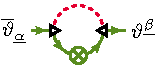
\includegraphics{0d/diagrams/SU2model0d-TwoPtFlow_20101_1.pdf}}\end{gathered}
-\,\begin{gathered}\raisebox{-3pt}{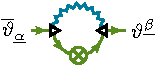
\includegraphics{0d/diagrams/SU2model0d-TwoPtFlow_20011_1.pdf}}\end{gathered}-\notag\\
&\qquad-\,\begin{gathered}\raisebox{-3pt}{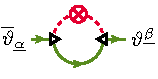
\includegraphics{0d/diagrams/SU2model0d-TwoPtFlow_10203_1.pdf}}\end{gathered}
-\,\begin{gathered}\raisebox{-3pt}{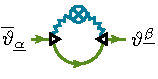
\includegraphics{0d/diagrams/SU2model0d-TwoPtFlow_10024_1.pdf}}\end{gathered}-\notag\\
&\qquad-\,\begin{gathered}\raisebox{-3pt}{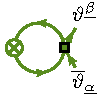
\includegraphics{0d/diagrams/SU2model0d-TwoPtFlow_20001_1.pdf}}\end{gathered}
-\frac{1}{2}\,\begin{gathered}\raisebox{-3pt}{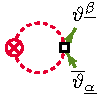
\includegraphics{0d/diagrams/SU2model0d-TwoPtFlow_00203_1.pdf}}\end{gathered}
-\frac{1}{2}\,\begin{gathered}\raisebox{-3pt}{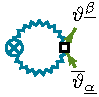
\includegraphics{0d/diagrams/SU2model0d-TwoPtFlow_00024_1.pdf}}\end{gathered}\, , \label{eq:SU2model0dG2tbt}
\end{align}
by means of appropriate contractions:
\begin{alignat}{2}
	\partial_t \FScoupling{Y}{0}{\sigma} &= \iu \suIItij{3}{\beta}{\alpha}\vts \partial_t\FSvertexArg{\FSeaaEoM}{\MFthetab_{{\alpha}},\MFtheta^{{\beta}}} &&= \FRGflow_t^Y\big[\sigma;\FScoupling{u}{0,1}{\sigma},\FScoupling{m}{0,1}{\sigma},\FScoupling{Y}{0,1,2}{\sigma},\FScoupling{g}{0}{\sigma}\big]
	\label{eq:SU2model0dYFlow}\,,\\[.2em]
	\partial_t \FScoupling{m}{0}{\sigma} &= -2 \suIItij{0}{\beta}{\alpha}\vts \partial_t\FSvertexArg{\FSeaaEoM}{\MFthetab_{{\alpha}},\MFtheta^{{\beta}}} &&= \FRGflow_t^{\vts m}\big[\sigma;\FScoupling{u}{0,1}{\sigma},\FScoupling{m}{0,1,2}{\sigma},\FScoupling{Y}{0,1}{\sigma},\FScoupling{g}{0}{\sigma}\big]
	\label{eq:SU2model0dmFlow}\,.
\end{alignat}
The flow \cref{eq:SU2model0dG2tbt} follows directly from traces over \cref{eq:FS2}.
The resulting expressions for $\FRGflow_t^Y$ and $\FRGflow_t^m$ are rather lengthy and can be found in Sec. 2.4 of our auxiliary notebook~\cite{Steil:2023zeroDSU2}.\bigskip

An important structural difference between the \frg{} flows $\FRGflow_t^Y[\ldots]$ and $\FRGflow_t^{\vts m}[\ldots]$ for the \gmv{} couplings and the one for the scalar self-interaction potential $\FRGflow_t^U[\ldots]$ is, that $\FRGflow_t^Y[\ldots]$ ($\FRGflow_t^{\vts m}[\ldots]$) includes a dependence on $\FScoupling{Y}{0}{\sigma}$ ($\FScoupling{m}{0}{\sigma}$) primarily \dash{} but not exclusively \dash{} due to the \gmv{} propagators, \cf{} \cref{app:SU2FSelements}.
This makes a naive conservation reformulation impossible.

The (re)formulation of conservative flow equations for field-dependent couplings like the Yukawa coupling $\FScoupling{h}{0}{\sigma} $ and the associated mass term $\FScoupling{Y}{0}{\sigma}$
is an open problem~\cite{\consYRef}.
We hope to gain new insights into the issue by further considering and massaging the the flow equations of zero-dimensional Grassmann-scalar models, like the $SU(2)$ model discussed here.

A rather interesting prospect in this context are alternative projections onto $\FScoupling{Y}{1}{\sigma}$ and $\FScoupling{m}{1}{\sigma}$.
Using the flow for the corresponding three-point function $\partial_t\FSvertexArg{\FSeaaEoM}{\MFthetab_{\underline{\alpha}},\MFtheta^{\underline{\beta}},\sigma}$ from \cref{eq:FS3} with appropriate contractions yields:
\begin{align}
\partial_t \FScoupling{Y}{1}{\sigma} &= \iu \suIItij{3}{\beta}{\alpha}\vts \partial_t\FSvertexArg{\FSeaaEoM}{\MFthetab_{{\alpha}},\MFtheta^{{\beta}},\sigma}\,=\notag\\* % no page break
&= \FRGflow_t^{\vts \partial_\sigma Y}\big[\sigma;\FScoupling{u}{0,1}{\sigma},\FScoupling{m}{0,1,2}{\sigma},\FScoupling{Y}{0,1,2,3}{\sigma},\FScoupling{g}{0,1}{\sigma}\big]
\label{eq:SU2model0dY1Flow}\,,\\[.2em]
\partial_t \FScoupling{m}{1}{\sigma} &= -2 \suIItij{0}{\beta}{\alpha}\vts \partial_t\FSvertexArg{\FSeaaEoM}{\MFthetab_{{\alpha}},\MFtheta^{{\beta}},\sigma}\,=\notag\\* % no page break
&= \FRGflow_t^{\vts \partial_\sigma m}\big[\sigma;\FScoupling{u}{0,1}{\sigma},\FScoupling{m}{0,1,2,3}{\sigma},\FScoupling{Y}{0,1,2}{\sigma},\FScoupling{g}{0,1}{\sigma}\big]
\label{eq:SU2model0dm1Flow}\,.
\end{align}
These flow equations might contain additional constraints since
\begin{align}
\partial_\sigma\FRGflow_t^{Y}[\ldots]\neq\FRGflow_t^{\vts \partial_\sigma Y}[\ldots]\,,\\
\partial_\sigma\FRGflow_t^{\vts m}[\ldots]\neq\FRGflow_t^{\vts \partial_\sigma m}[\ldots]\,,
\end{align}
which one might be able to use to facilitate the construction of conservative flow equations for $\FScoupling{Y}{1}{\sigma}$ and $\FScoupling{m}{1}{\sigma}$.
This is however still subject of ongoing research and development.

\paragraph{Flow equation for the four-Grassmann coupling \texorpdfstring{$g_t(\sigma)$}{g}}\phantomsection\label{paragraph:0dSU2flowh}\mbox{}\\%
The flow equations for the four-Grassmann coupling \texorpdfstring{$g_t(\sigma)$}{g} can be obtained from the flow \cref{eq:FS4} for the corresponding four-point function by means of appropriate contractions:
\begin{align}
\partial_t g_t(\sigma)&=%
-8\suIItij{0}{\gamma}{\beta} \suIItij{0}{\delta}{\alpha}\vts\FSvertexArg{\FSeaaEoM}{\overline{\vartheta} {}_{{\delta}},{\vartheta} \text{}^{{\gamma}},\overline{\vartheta} {}_{{\beta}},{\vartheta} \text{}^{{\alpha}}}\,=\notag\\*[,1em] % no page break
&=\FRGflow_t^g\big[\sigma;\FScoupling{u}{0,1}{\sigma},\FScoupling{m}{0,1,2}{\sigma},\FScoupling{Y}{0,1,2}{\sigma},\FScoupling{g}{0,1,2}{\sigma}\big]\label{eq:SU2model0dhFlow} \\[.2em]
\newEqBlockPrime
&=-4\,\begin{gathered}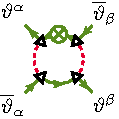
\includegraphics{0d/diagrams/SU2model0d-FourPtFlowTr_30201_1.pdf}\end{gathered}+\skeleton{1}
-4\,\begin{gathered}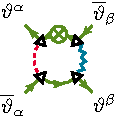
\includegraphics{0d/diagrams/SU2model0d-FourPtFlowTr_30111_1.pdf}\end{gathered}+\skeleton{3}
-4\,\begin{gathered}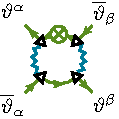
\includegraphics{0d/diagrams/SU2model0d-FourPtFlowTr_30021_1.pdf}\end{gathered}+\skeleton{1}-\notag\\ 
&\quad-4\,\begin{gathered}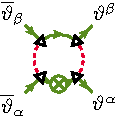
\includegraphics{0d/diagrams/SU2model0d-FourPtFlowTr_21201_1.pdf}\end{gathered}+\skeleton{1}
-4\,\begin{gathered}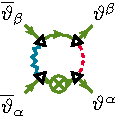
\includegraphics{0d/diagrams/SU2model0d-FourPtFlowTr_21111_1.pdf}\end{gathered}+\skeleton{3}
-4\,\begin{gathered}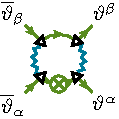
\includegraphics{0d/diagrams/SU2model0d-FourPtFlowTr_21021_1.pdf}\end{gathered}+\skeleton{1}-\notag\\ 
&\quad-4\,\begin{gathered}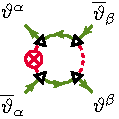
\includegraphics{0d/diagrams/SU2model0d-FourPtFlowTr_20303_1.pdf}\end{gathered}+\skeleton{1}
-4\,\begin{gathered}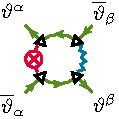
\includegraphics{0d/diagrams/SU2model0d-FourPtFlowTr_20213_1.pdf}\end{gathered}+\skeleton{1}
-4\,\begin{gathered}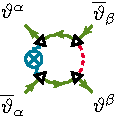
\includegraphics{0d/diagrams/SU2model0d-FourPtFlowTr_20124_1.pdf}\end{gathered}+\skeleton{1}-\notag\\ 
&\quad-4\,\begin{gathered}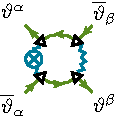
\includegraphics{0d/diagrams/SU2model0d-FourPtFlowTr_20034_1.pdf}\end{gathered}+\skeleton{1}
-2\,\begin{gathered}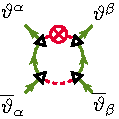
\includegraphics{0d/diagrams/SU2model0d-FourPtFlowTr_11303_1.pdf}\end{gathered}+\skeleton{3}
-2\,\begin{gathered}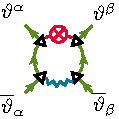
\includegraphics{0d/diagrams/SU2model0d-FourPtFlowTr_11213_1.pdf}\end{gathered}+\skeleton{3}-\notag\\ 
&\quad-2\,\begin{gathered}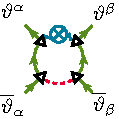
\includegraphics{0d/diagrams/SU2model0d-FourPtFlowTr_11124_1.pdf}\end{gathered}+\skeleton{3}
-2\,\begin{gathered}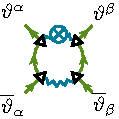
\includegraphics{0d/diagrams/SU2model0d-FourPtFlowTr_11034_1.pdf}\end{gathered}+\skeleton{3}
-2\,\begin{gathered}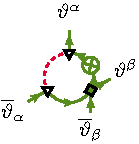
\includegraphics{0d/diagrams/SU2model0d-FourPtFlowTr_30101_1.pdf}\end{gathered}+\skeleton{5}-\notag\\ 
&\quad-2\,\begin{gathered}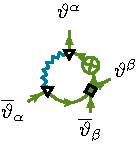
\includegraphics{0d/diagrams/SU2model0d-FourPtFlowTr_30011_1.pdf}\end{gathered}+\skeleton{5}
-2\,\begin{gathered}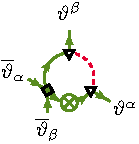
\includegraphics{0d/diagrams/SU2model0d-FourPtFlowTr_21101_1.pdf}\end{gathered}+\skeleton{3}
-2\,\begin{gathered}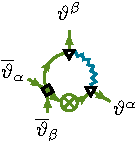
\includegraphics{0d/diagrams/SU2model0d-FourPtFlowTr_21011_1.pdf}\end{gathered}+\skeleton{3}-\notag\\ 
&\quad-4\,\begin{gathered}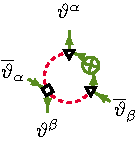
\includegraphics{0d/diagrams/SU2model0d-FourPtFlowTr_20201_1.pdf}\end{gathered}+\skeleton{2}
-2\,\begin{gathered}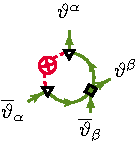
\includegraphics{0d/diagrams/SU2model0d-FourPtFlowTr_20203_1.pdf}\end{gathered}+\skeleton{2}
-4\,\begin{gathered}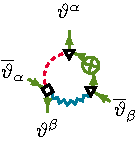
\includegraphics{0d/diagrams/SU2model0d-FourPtFlowTr_20111_1.pdf}\end{gathered}+\skeleton{5}-\notag\\ 
&\quad-4\,\begin{gathered}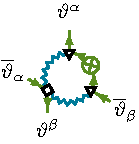
\includegraphics{0d/diagrams/SU2model0d-FourPtFlowTr_20021_1.pdf}\end{gathered}+\skeleton{2}
-2\,\begin{gathered}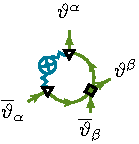
\includegraphics{0d/diagrams/SU2model0d-FourPtFlowTr_20024_1.pdf}\end{gathered}+\skeleton{2}
-\,\begin{gathered}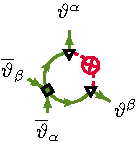
\includegraphics{0d/diagrams/SU2model0d-FourPtFlowTr_11203_1.pdf}\end{gathered}+\skeleton{3}-\notag\\ 
&\quad-\,\begin{gathered}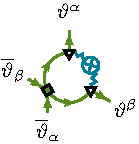
\includegraphics{0d/diagrams/SU2model0d-FourPtFlowTr_11024_1.pdf}\end{gathered}+\skeleton{3}
-4\,\begin{gathered}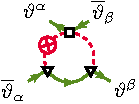
\includegraphics{0d/diagrams/SU2model0d-FourPtFlowTr_10303_1.pdf}\end{gathered}+\skeleton{5}
-4\,\begin{gathered}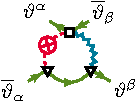
\includegraphics{0d/diagrams/SU2model0d-FourPtFlowTr_10213_1.pdf}\end{gathered}+\skeleton{5}-\notag\\ 
&\quad-4\,\begin{gathered}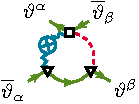
\includegraphics{0d/diagrams/SU2model0d-FourPtFlowTr_10124_1.pdf}\end{gathered}+\skeleton{5}
-4\,\begin{gathered}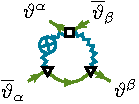
\includegraphics{0d/diagrams/SU2model0d-FourPtFlowTr_10034_1.pdf}\end{gathered}+\skeleton{5}
+2\,\begin{gathered}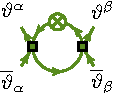
\includegraphics{0d/diagrams/SU2model0d-FourPtFlowTr_30001_1.pdf}\end{gathered}+\skeleton{2}-\notag\\ 
&\quad-2\,\begin{gathered}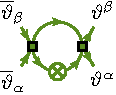
\includegraphics{0d/diagrams/SU2model0d-FourPtFlowTr_21001_1.pdf}\end{gathered}
+2\,\begin{gathered}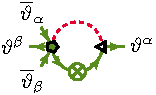
\includegraphics{0d/diagrams/SU2model0d-FourPtFlowTr_20101_1.pdf}\end{gathered}+\skeleton{3}
+2\,\begin{gathered}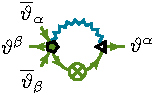
\includegraphics{0d/diagrams/SU2model0d-FourPtFlowTr_20011_1.pdf}\end{gathered}+\skeleton{3}+\notag\\ 
&\quad+2\,\begin{gathered}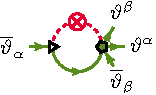
\includegraphics{0d/diagrams/SU2model0d-FourPtFlowTr_10203_1.pdf}\end{gathered}+\skeleton{3}
+2\,\begin{gathered}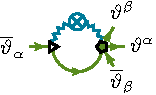
\includegraphics{0d/diagrams/SU2model0d-FourPtFlowTr_10024_1.pdf}\end{gathered}+\skeleton{3}-\notag\\
&\quad-2\,\begin{gathered}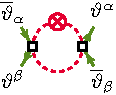
\includegraphics{0d/diagrams/SU2model0d-FourPtFlowTr_00303_1.pdf}\end{gathered}+\skeleton{2}
-2\,\begin{gathered}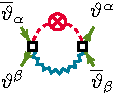
\includegraphics{0d/diagrams/SU2model0d-FourPtFlowTr_00213_1.pdf}\end{gathered}+\skeleton{2}
+\,\begin{gathered}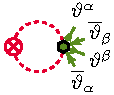
\includegraphics{0d/diagrams/SU2model0d-FourPtFlowTr_00203_1.pdf}\end{gathered}-\notag\\
&\quad-2\,\begin{gathered}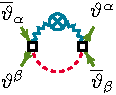
\includegraphics{0d/diagrams/SU2model0d-FourPtFlowTr_00124_1.pdf}\end{gathered}+\skeleton{2}
-2\,\begin{gathered}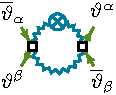
\includegraphics{0d/diagrams/SU2model0d-FourPtFlowTr_00034_1.pdf}\end{gathered}+\skeleton{2}
+\,\begin{gathered}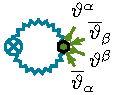
\includegraphics{0d/diagrams/SU2model0d-FourPtFlowTr_00024_1.pdf}\end{gathered}\, , \eqTagPrime 
\end{align}
where the following six classes of diagrams vanish,
\begin{align}
0 &= %
-4\,\begin{gathered}\includegraphics{0d/diagrams/SU2model0d-FourPtFlowTr_30201_1.pdf}\end{gathered}+\skeleton{1} \, =
-4\,\begin{gathered}\includegraphics{0d/diagrams/SU2model0d-FourPtFlowTr_20303_1.pdf}\end{gathered}+\skeleton{1} \, =\notag\\
&=-2\,\begin{gathered}\includegraphics{0d/diagrams/SU2model0d-FourPtFlowTr_30101_1.pdf}\end{gathered}+\skeleton{5} \, =
-2\,\begin{gathered}\includegraphics{0d/diagrams/SU2model0d-FourPtFlowTr_20203_1.pdf}\end{gathered}+\skeleton{2} \, =\notag\\
&=+2\,\begin{gathered}\includegraphics{0d/diagrams/SU2model0d-FourPtFlowTr_20101_1.pdf}\end{gathered}+\skeleton{3} \, =
+2\,\begin{gathered}\includegraphics{0d/diagrams/SU2model0d-FourPtFlowTr_10203_1.pdf}\end{gathered}+\skeleton{3}
\label{eq:SU2model0dh0}\, ,
\end{align}
after tracing in flavor space.
Thus from the 41 classes of diagrams in \cref{eq:SU2model0dhFlow}, 35 have non-vanishing contributions.
The resulting expression for $\FRGflow_t^g$ is very lengthy and can be found in Sec. 2.5 of our auxiliary notebook~\cite{Steil:2023zeroDSU2}.\bigskip

As for the flow \cref{eq:SU2model0dYFlow,eq:SU2model0dmFlow} a conservative formulation for the flow equation for the field-dependent four-Grassmann coupling $\partial_t g_t(\sigma)$ is also not obvious due to the dependence $\FRGflow_t^g[\ldots,\FScoupling{g}{0}{\sigma},\ldots]$.
An alternative projection onto $\FScoupling{g}{1}{\sigma}$ by means of the flow for the corresponding five-point function with an appropriate contraction
\begin{align}
\partial_t g_t(\sigma)&=%
-8\suIItij{1}{\gamma}{\beta} \suIItij{0}{\delta}{\alpha}\vts\FSvertexArg{\FSeaaEoM}{\overline{\vartheta} {}_{{\delta}},{\vartheta} \text{}^{{\gamma}},\overline{\vartheta} {}_{{\beta}},{\vartheta} \text{}^{{\alpha}},\sigma}\,=\notag\\*[,1em] % no page break
&=\FRGflow_t^g\big[\sigma;\FScoupling{u}{0,1}{\sigma},\FScoupling{m}{0,1,2,3}{\sigma},\FScoupling{Y}{0,1,2,3}{\sigma},\FScoupling{g}{0,1,2,3}{\sigma}\big]\label{eq:SU2model0dh1Flow}\,,
\end{align}
might again be worthwhile to consider, since
\begin{align}
\partial_\sigma\FRGflow_t^{g}[\ldots]\neq\FRGflow_t^{\vts \partial_\sigma g}[\ldots]\,.
\end{align}

We will refrain from further discussions at this point and refer to the following outlook~\ref{paragraph:0dconclusionFermions}.
\renewcommand{\FSk}{k}